In general we will not be so lucky as to have a problem with linear-Gaussian dynamics. In this case, a particle filter (PF) may be the best alternative. The PF is based on the idea that if we cannot represent a probability distribution analytically then we may approximate it as a collection of discrete samples or ``particles'' drawn from the distribution.

\begin{figure}[!hbt] \centering
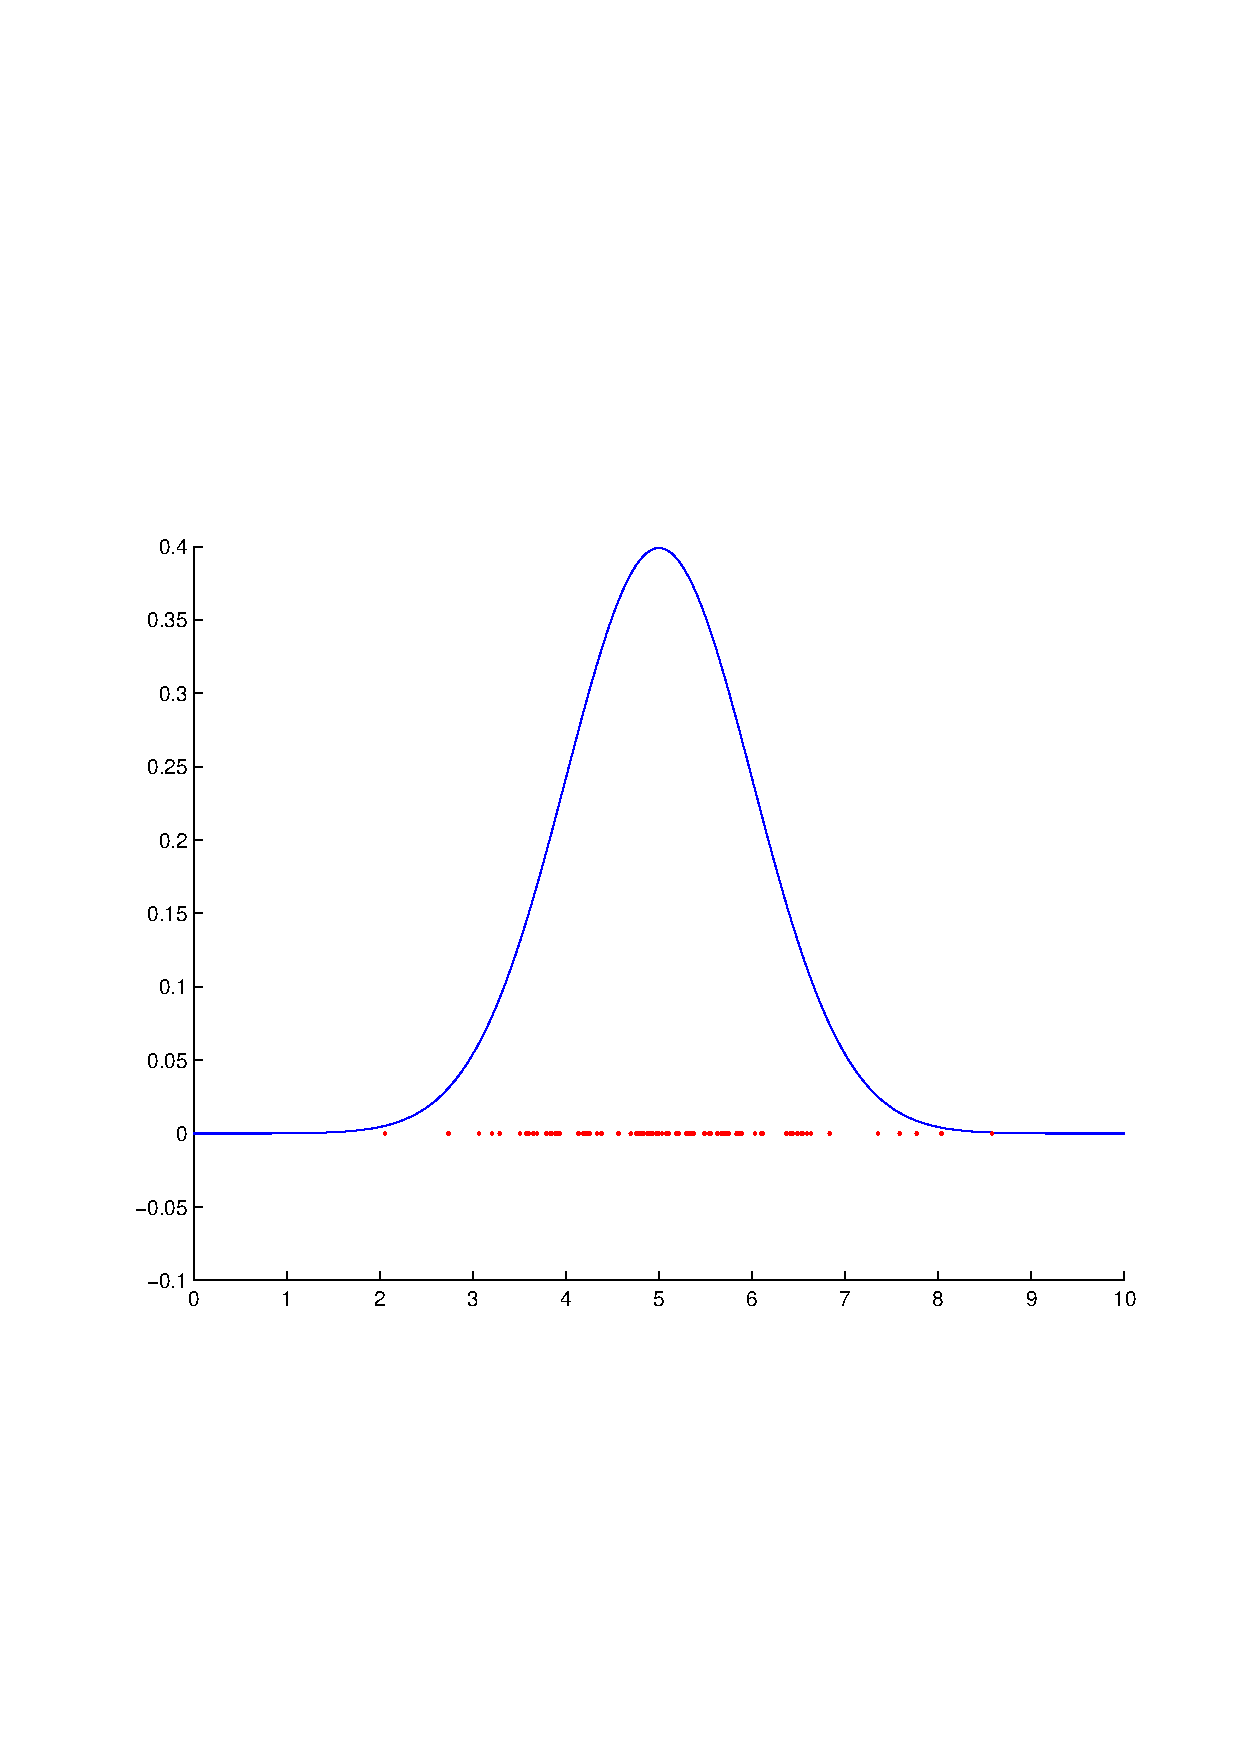
\includegraphics[width=0.7\columnwidth]{MonteCarlo.pdf}%
\caption{An analytic probability density (blue) may be approximated by a set of samples drawn from it (red)}%
\label{fig:MonteCarlo}%
\end{figure}

Often, it will not even be possible to sample from the desired distribution. We therefore use importance sampling (IS) or Markov chain Monte Carlo methods to generate these samples. The principle of a particle filter is that we recursively generate such a set of particles to approximate $P(X_{1:t}|Y_{1:t})$ given a previous set representing $P(X_{1:t-1}|Y_{1:t-1})$.

\subsection{The basics}

With a PF, we approximate a probability distribution with a set of (weighted) samples drawn from that distribution.

\begin{equation}
P(X) \approx \frac{1}{N} \sum_m{W^{(m)} \delta_{X^{(m)}} (X)}
\label{eq:ParticleApprox}
\end{equation}

where $\delta (x)$ represents a unit probability point mass at a point $x$, and $\sum_m{W^{(m)}}=1$. Such a method allows us to represent any probability distribution of arbitrary complexity, including multidimensional, multimodal, mixed distributions. As the number of particles increases, the accuracy of the approximation improves at the expense of computational complexity. Thus we have the required tool for estimation in non-linear, non-Gaussian scenarios.

We still face the problem of how to generate these samples. The conventional method for this is Sequential Importance Sampling with Resampling (SISR). For a more complete and traditional introduction to this method, see \cite{Cappe2007} or \cite{Doucet2009}. Here we follow an outline similar to that used for the derivation of the auxiliary particle filter of \cite{Pitt1999}.

Suppose we have a particle approximation to the joint posterior distribution from the previous frame, $\hat{P}(X_{1:t-1}|Y_{1:t-1})$. Each particle represents a path through time, $X_{1:t-1}^{(m)}$, and has an associated weight, $W_{t-1}^{(m)}$. Let us suppose also that the unweighted particles may be considered samples from another distribution:

\begin{equation}
\mu(X_{1:t-1}|Y_{1:t-1}) \approx \frac{1}{N} \sum_m{W^{(m)} \delta_{X_{1:t}^{(m)}} (X_{1:t})}
\label{eq:UnweightParticleDistn}
\end{equation}

Thus for a given particle,

\begin{equation}
\hat{P}(X_{1:t-1}^{(m)}|Y_{1:t-1}) = W_t^{(m)} \mu(X_{1:t-1}^{(m)}|Y_{1:t-1})
\label{eq:}
\end{equation}

We would like to generate a new particle set which includes the current time instance. We propose a new set of extended tracks from a factored proposal distribution $X_{1:t} \sim q(X_{1:t}|Y_{1:t}) = q(X_{t}|Y_{t}, X_{1:t-1}) q(X_{1:t-1}|Y_{1:t})$. The two factors are the proposal probabilities for the new state value, $X_t$ and the history, $X_{1:t-1}$, respectively. Particles are then weighted to take account of the difference between the targeted posterior distribution and the importance distribution:

\begin{equation}
W_t^{(m)} = \frac{P(X_{1:t}^{(m)}|Y_{1:t})}{q(X_{1:t}^{(m)}|Y_{1:t})}
\label{eq:ImportanceWeights}
\end{equation}

The simplest choice for the history proposal is $q(X_{1:t-1}|Y_{1:t}) = \mu(X_{1:t-1}|Y_{1:t-1})$, which can be implemented by simply keeping the same set of paths as the previous particle set. This is equivalent to an ordinary IS step with no resampling, and importance weights are given by:

\begin{equation}
W_t^{(m)} = \frac{P(X_{1:t}^{(m)}|Y_{1:t})}{q(X_{1:t}^{(m)}|Y_{1:t})}
\approx \frac{W_{t-1}^{(m)}P(X_{1:t}^{(m)}|Y_{1:t})}{P(X_{1:t-1}^{(m)}|Y_{1:t-1}) q(X_{t}^{(m)}|X_{t-1}^{(m)}, Y_{t})}
\propto \frac{W_{t-1}^{(m)} P(Y_t|X_t^{(m)})P(X_t^{(m)}|X_{t-1}^{(m)})}{q(X_t^{(m)}|X_{t-1}^{(m)}, Y_t)}
\label{eq:NoResampIW}
\end{equation}

Alternatively, we could use $q(X_{1:t-1}|Y_{1:t}) = \hat{P}(X_{1:t-1}|Y_{1:t-1})$ as the history proposal, i.e. sample from the weighted particle distribution which approximates the previous posterior. This is equivalent to an IS step preceeded by resampling. Importance weights are now given by:

\begin{equation}
W_t^{(m)} = \frac{P(X_{1:t}^{(m)}|Y_{1:t})}{q(X_{1:t}^{(m)}|Y_{1:t})}
\approx \frac{P(X_{1:t}^{(m)}|Y_{1:t})}{P(X_{1:t-1}^{(m)}|Y_{1:t-1}) q(X_{t}^{(m)}|X_{t-1}^{(m)}, Y_{t})}
\propto \frac{ P(Y_t|X_t^{(m)})P(X_t^{(m)}|X_{t-1}^{(m)})}{q(X_t^{(m)}|X_{t-1}^{(m)}, Y_t)}
\label{eq:WithResampIW}
\end{equation}


\subsection{Auxiliary sampling}

We can generalise the form of our history proposal distribution by weighting the particles from the previous posterior distribution with any arbitrary set of weights.

\begin{equation}
q(X_{1:t-1}|Y_{1:t}) = \frac{1}{N} \sum_m {V_t^{(m)} \delta_{X} (x_{1:t}^{(m)})}
\label{eq:AuxiliarySamplingProposal}
\end{equation}

Now we have

\begin{equation}
\hat{P}(X_{1:t-1}^{(m)}|Y_{1:t-1}) = \frac{W_{t-1}^{(m)}}{V_t^{(m)}} q(X_{1:t-1}^{(m)}|Y_{1:t})
\label{eq:}
\end{equation}

giving a general form for the importance weights

\begin{multline}
W_t^{(m)} = \frac{P(X_{1:t}^{(m)}|Y_{1:t})}{q(X_{1:t}^{(m)}|Y_{1:t})}
\approx \frac{W_{t-1}^{(m)}}{V_{t}^{(m)}} \times \frac{P(X_{1:t}^{(m)}|Y_{1:t})}{P(X_{1:t-1}^{(m)}|Y_{1:t-1}) q(X_{t}^{(m)}|X_{t-1}^{(m)}, Y_{t})}\\
\propto \frac{W_{t-1}^{(m)}}{V_{t}^{(m)}} \times \frac{ P(Y_t|X_t^{(m)})P(X_t^{(m)}|X_{t-1}^{(m)})}{q(X_t^{(m)}|X_{t-1}^{(m)}, Y_t)}
\label{eq:AuxiliaryIW}
\end{multline}

A suitable choice for the auxiliary proposal weights is the predictive likelihood of the next measurement, i.e.

\begin{equation}
V_t^{(m)} = P(Y_t|X_{t-1}^{(m)})
\label{eq:}
\end{equation}

This favours the selection of particles which better explain the new observation. This quantity is often not easily calculable, so approximations may be used, for example using a Gaussian approximation.



\subsection{Degeneracy and resampling}
The simplest history proposal is given by $q(X_{1:t-1}|Y_{1:t}) = \mu(X_{1:t-1}|Y_{1:t-1})$. This may be `sampled' by simply keeping the $N$ particles from the previous processing step, which is thus equivalent to importance sampling with no resampling. Multiple steps of this nature will lead to a fall in particle diversity, as many of the weights tend towards 0. This occurs because of the recursive nature of the importance weight calculation in equation~\ref{eq:NoResamIW}. The solution to this degeneracy is to use the other form of history proposal, $q(X_{1:t-1}|Y_{1:t}) = \hat{P}(X_{1:t-1}|Y_{1:t-1})$, equivalent to importance sampling with resampling. Such a proposal will require additional computation time, but the weight updates are no longer recursive, see equation~\ref{eq:ResamIW}, so diversity is improved.

The resampling/history-sampling may be conducted in a variety of ways. The simplest is multinomial sampling, in which each particle is sampled independently with replacement. In residual sampling, particles are sampled from the particle distribution without replacement, i.e. after a particle is selected, the probability of selecting it again is reduced. Finally, for systematic resampling, a finite real line is divided into sections corresponding to the weight of each particle. Particles are sampled by choosing regular points along this line, with some constant, random offset. The final method produces the least variance in the number of child particles chosen from each parent given the weights, and thus introduces the least Monte Carlo error. For more details see \cite{Doucet2009} and the references therein.

Degeneracy is measured using the Effective Sample Size of \cite{Liu1995}, which is given by:

\begin{equation}
ESS = \frac{1}{N} \sum_m W^{(m)2}
\label{eq:ESS}
\end{equation}

where $W^{(m)}$ are the particle weights, and there are $N$ particles. If ESS falls below some chosen threshold, resampling this required to replenish particle diversity.



\subsection{Importance distributions}

It remains to choose the the importance distribution for the current state, $q(X_{t}|X_{t-1}, Y_{t})$. In the original ``bootstrap filter'' of \cite{Gordon1993}, this was set equal to the transition density, $P(X_t|X_{t-1})$, which leads to cancellation in the expression for importance weights. This is simple but not necessarily optimal. For example if the process noise is high, the samples of $X_t$ will be widely spread. If, however, the observation noise is comparitively low, many or most of the samples will be far from the observation and will have a low weight, giving us poor particle diversity.

An improved choice of proposal distribution is given by:

\begin{equation}
q(X_{t}|X_{t-1}, Y_{t}) = P(X_t|X_{t-1}, Y_t) = \frac{P(Y_t|X_t)P(X_t|X_{t-1})}{P(Y_t|X_{t-1})}
\label{eq:OptimalImportanceDist}
\end{equation}

This is often known as the ``optimal importance distribution''. The importance weights for a step without resampling are now given by:

\begin{equation}
W_t^{(m)} \propto \frac{ W_{t-1}^{(m)} }{ V_t^{(m)} } \times \frac{ P(Y_t|X_t^{(m)})P(X_t^{(m)}|X_{t-1}^{(m)}) }{q(X_t^{(m)}|X_{t-1}^{(m)}, Y_t)} \propto \frac{ W_{t-1}^{(m)} }{ V_t^{(m)} } \times P(Y_t|X_{t-1}^{(m)})
\label{eq:OptimalImportanceWeights}
\end{equation}

If the auxiliary weights are set to $V_t^{(m)}=P(Y_t|X_{t-1}^{(m)})$ then all weights are equal throughout, and resampling will never be required. In general, the optimal importance distribution will not be samplable, but proposals using Gaussian approximations of this form may be used.